\chapter{Настройка и обслуживание \ReplicaGenOne{}}\label{ch:replica-setup-ru}

Эта глава относится к классической приборке \ReplicaGenOne{}, показанной на \autoref{fig:replica-classic-ru}. Если ваша панель соответствует компоновке \ReplicaNextLong{}, воспользуйтесь предыдущим разделом.

\begin{figure}[htbp]
    \centering
    \begin{subfigure}{0.46\textwidth}
        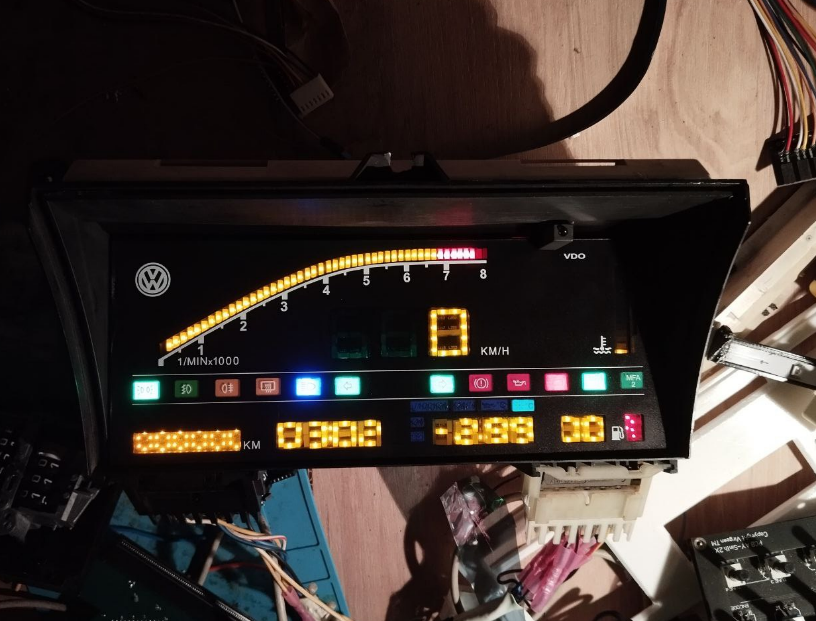
\includegraphics[width=\linewidth]{digifiz_manual/image046.png}
        \caption{Классическая \ReplicaGenOne{} с квадратной рамкой.}
    \end{subfigure}\hfill
    \begin{subfigure}{0.46\textwidth}
        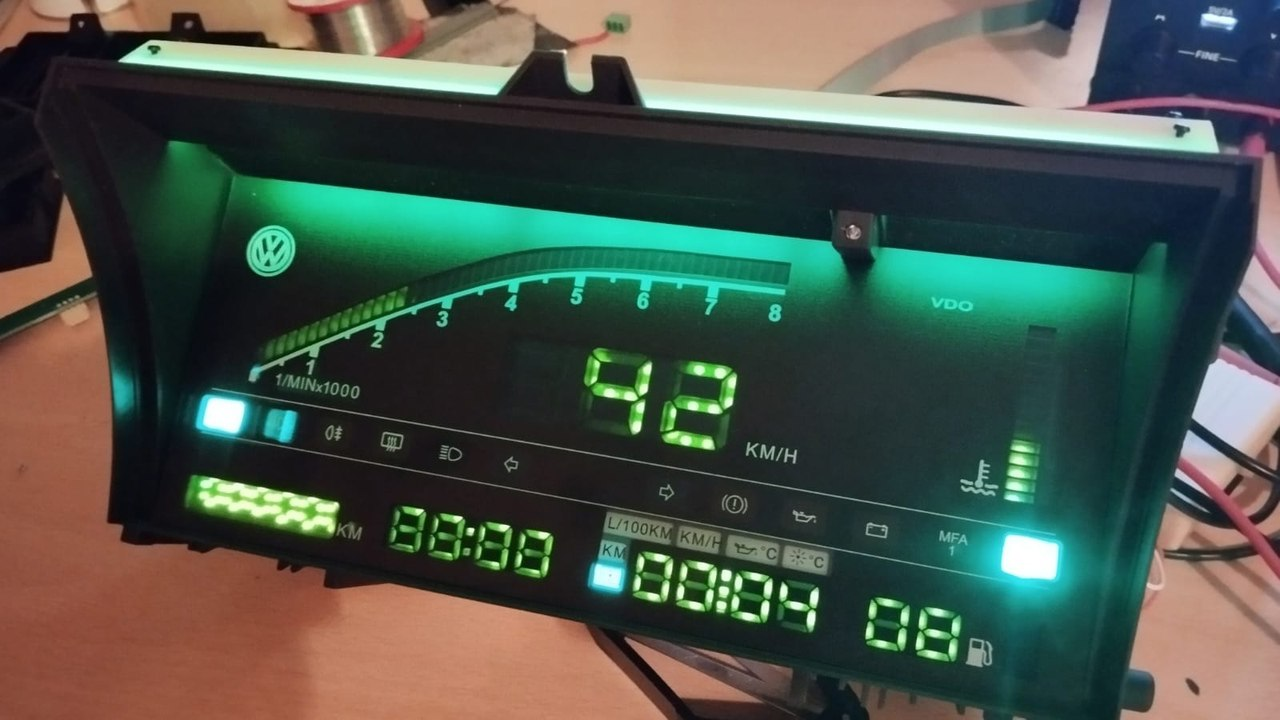
\includegraphics[width=\linewidth]{digifiz_manual/image047.png}
        \caption{Закруглённая рамка поздних комплектов.}
    \end{subfigure}
    \caption{Внешний вид приборной панели \ReplicaGenOne{}.}
    \label{fig:replica-classic-ru}
\end{figure}

\section{Уход за экраном}
\begin{itemize}
    \item Передняя панель из оргстекла с УФ-печатью легко царапается. Избегайте контакта с острыми или абразивными предметами.
    \item Поверхностные повреждения являются косметическими и не покрываются гарантией. При деформации рисунка заказывайте запасные детали у PHOL-LABS Kft.
\end{itemize}

\section{Батарея часов реального времени}
Внутри установлен модуль DS3231 с элементом CR2032. Обычно батарея служит около четырёх лет.
Когда она разряжается, часы сбрасываются при каждом включении.
Снимите переднюю и/или заднюю крышку, не отключая жгуты, и замените элемент питания. Утилизируйте использованную батарейку согласно местным правилам.

\section{Обновление прошивки через USBasp}
Каждый комплект включает кабель программатора USBasp, уже подключённый внутри корпуса (\autoref{fig:usbasp-cable-ru}).
Перед прошивкой установите драйвер USBasp, например, скачав его по ссылке:
\displayurl{https://myrobot.ru/downloads/driver-usbasp-v-2.0-usb-isp-windows-7-8-10-xp.php}
При подключении программатор питает приборку, что позволяет выполнять проверки на стенде.

\begin{figure}[htbp]
    \centering
    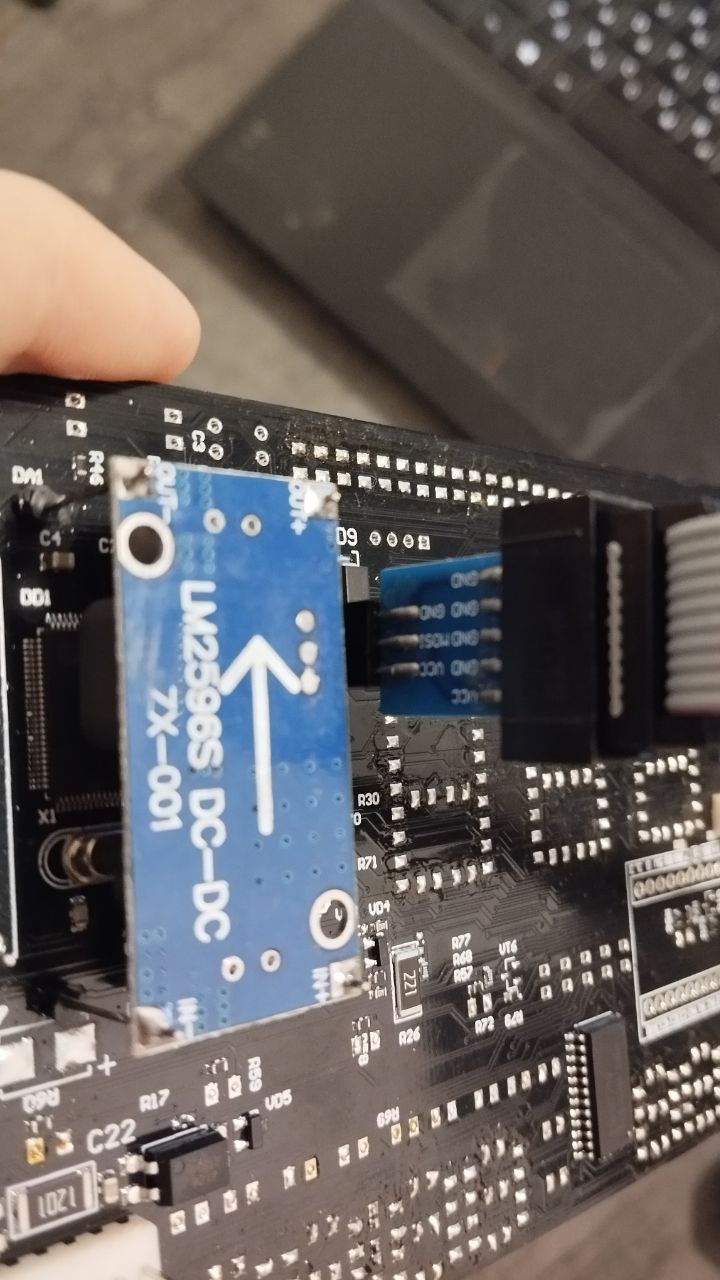
\includegraphics[width=0.32\textwidth]{digifiz_manual/image048.png}
    \caption{Ориентация шлейфа USBasp внутри \ReplicaGenOne{}.}
    \label{fig:usbasp-cable-ru}
\end{figure}

Прошивку выполняйте командой \texttt{avrdude} (при необходимости измените имя файла прошивки):

\begin{verbatim}
avrdude -c usbasp -p m2560 -e \
    -U lfuse:w:0xff:m -U hfuse:w:0x99:m -U efuse:w:0xff:m \
    -U flash:w:Digifiz.ino.mega.hex
\end{verbatim}

После успешной записи коснитесь фронтальной сенсорной кнопки 4--5 раз, чтобы инициализировать блоки памяти.
Если они остаются пустыми, повторите прошивку или отправьте Bluetooth-команду \verb|252 0| для заводского сброса.
Готовые образы прошивки опубликованы здесь:
\displayurl{https://github.com/Sgw32/DigifizReplica}

\section{Конфигурация по Bluetooth}
Большинство параметров настраиваются по Bluetooth с Android-смартфона и приложением Serial Bluetooth Terminal.
Скачайте его по ссылке перед сопряжением с приборкой:
\displayurl{https://play.google.com/store/apps/details?id=de.kai_morich.serial_bluetooth_terminal&hl=en&gl=US}
Устройства iOS не поддерживают модуль Bluetooth 2.0.

\begin{itemize}
    \item Сопрягайтесь именно с интерфейсом Bluetooth Classic приборки, избегая устройств, работающих только через BLE.
    \item В Serial Bluetooth Terminal установите символ конца строки LF и отключите режим CR+LF перед отправкой команд.
\end{itemize}

\begin{figure}[htbp]
    \centering
    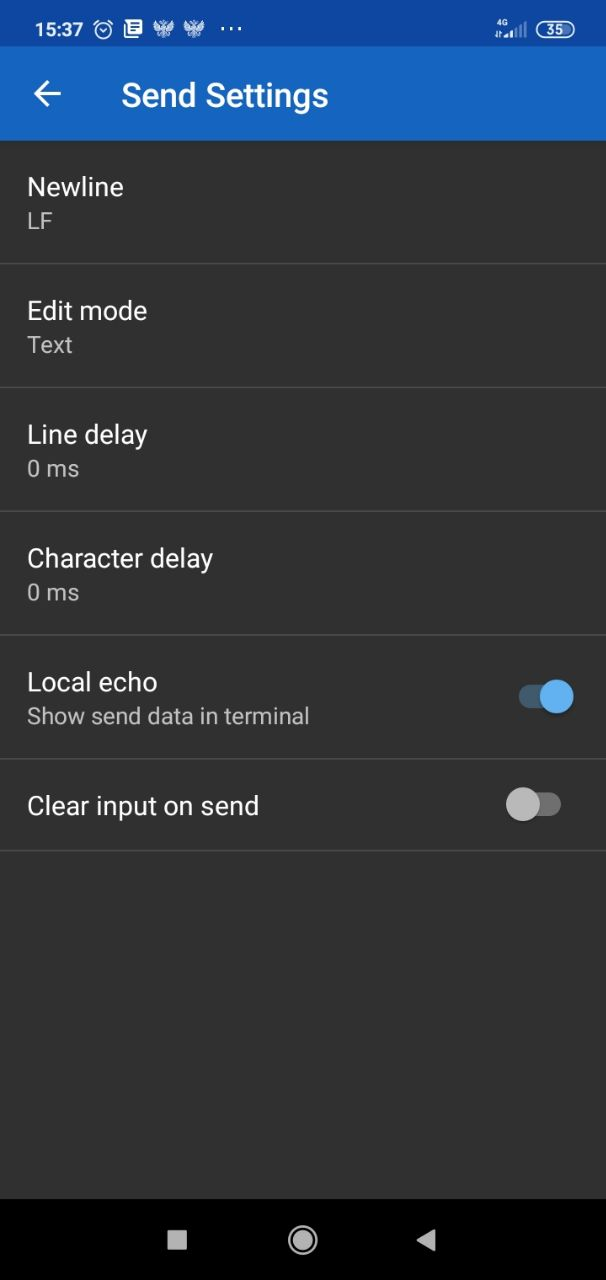
\includegraphics[width=0.32\textwidth]{digifiz_manual/image049.png}
    \caption{Рекомендуемые настройки Serial Bluetooth Terminal.}
    \label{fig:sbt-settings-ru}
\end{figure}

Команды вводятся парами \verb|<номер> <значение>|.
Например, чтобы записать пробег 123\,456~км, отправьте \verb|11 123456|.
Чтобы прочитать текущее значение, прибавьте 128 к номеру команды (\verb|129 0| возвращает коэффициент скорости).
Диагностическая команда \verb|adc 0| выводит сырые данные датчиков для анализа неисправностей.

\section{Параметры конфигурации}
Основные Bluetooth-команды перечислены в \autoref{tbl:replica-classic-commands-ru}.
Значения по умолчанию для приборок поколений~1/1.5 и 2 приведены в \autoref{tbl:replica-defaults-ru}.
Команды 31--33 применимы только к \ReplicaNextShort{} и не влияют на классическую \ReplicaGenOneShort{}.

{\scriptsize
\begin{longtblr}[
    caption = {Команды конфигурации классической \ReplicaGenOne{}.},
    label = {tbl:replica-classic-commands-ru},
]{
    colspec = {Q[c,0.14\linewidth] >{\ttfamily}Q[l,0.38\linewidth] Q[l]},
    rowsep = 2pt,
}
    \toprule
    \textbf{ID} & \textbf{Name} & \textbf{Описание} \\
    \midrule
    22 (или 0) & PARAMETER\_RPMCOEFFICIENT & Калибровочный коэффициент оборотов. \\
    1 & PARAMETER\_SPEEDCOEFFICIENT & Калибровка скорости. \\
    2 & PARAMETER\_COOLANTTHERMISTORB & Бета-коэффициент датчика ОЖ. \\
    3 & PARAMETER\_OILTHERMISTORB & Бета-коэффициент датчика масла. \\
    4 & PARAMETER\_AIRTHERMISTORB & Бета-коэффициент датчика наружной температуры. \\
    5 & PARAMETER\_TANKMINRESISTANCE & Минимальное сопротивление датчика топлива (\si{\ohm}). \\
    6 & PARAMETER\_TANKMAXRESISTANCE & Максимальное сопротивление датчика топлива (\si{\ohm}). \\
    7 & PARAMETER\_TAU\_COOLANT & Постоянная фильтра температуры ОЖ. \\
    8 & PARAMETER\_TAU\_OIL & Постоянная фильтра температуры масла. \\
    9 & PARAMETER\_TAU\_AIR & Постоянная фильтра наружной температуры. \\
    10 & PARAMETER\_TAU\_TANK & Постоянная фильтра уровня топлива. \\
    11 & PARAMETER\_MILEAGE & Общий пробег. \\
    12 & PARAMETER\_DAILY\_MILEAGE & Суточный пробег. \\
    13 & PARAMETER\_AUTO\_BRIGHTNESS & Включение автоматической яркости. \\
    14 & PARAMETER\_BRIGHTNESS\_LEVEL & Ручной уровень яркости (0--15). \\
    15 & PARAMETER\_TANK\_CAPACITY & Ёмкость бака (литры). \\
    16 & PARAMETER\_MFA\_STATE & Активная страница MFA. \\
    17 & PARAMETER\_BUZZER\_OFF & Отключение зуммера (1 — выкл., 0 — вкл.). \\
    18 & PARAMETER\_MAX\_RPM & Диапазон тахометра (по умолчанию 8000). \\
    19 & PARAMETER\_NORMAL\_RESISTANCE\_COOLANT & Сопротивление датчика ОЖ при \SI{25}{\celsius}. \\
    20 & PARAMETER\_NORMAL\_RESISTANCE\_OIL & Сопротивление датчика масла при \SI{25}{\celsius}. \\
    21 & PARAMETER\_NORMAL\_RESISTANCE\_AMB & Сопротивление датчика наружного воздуха при \SI{25}{\celsius}. \\
    23 & PARAMETER\_DOT\_OFF & Поведение разделителя часов (0 — мигает, 1 — постоянно). \\
    24 & PARAMETER\_BACKLIGHT\_ON & Включение подсветки при ближнем свете. \\
    25 & PARAMETER\_M\_D\_FILTER & Константа медианного фильтра (наследие). \\
    26 & PARAMETER\_COOLANT\_MAX\_R & Порог полной шкалы температуры ОЖ. \\
    27 & PARAMETER\_COOLANT\_MIN\_R & Порог «1~bar» температуры ОЖ. \\
    31--33 & PARAMETER\_MAINCOLOR\_[RGB] & Компоненты цвета интерфейса (только \ReplicaNextShort{}). \\
    37 & PARAMETER\_RPM\_FILTER & Агрессивность фильтра оборотов. \\
    128 & PARAMETER\_READ\_ADDITION & Добавьте для чтения параметра. \\
    255 & PARAMETER\_SET\_HOUR & Установка часов (24-часовой формат). \\
    254 & PARAMETER\_SET\_MINUTE & Установка минут. \\
    253 & PARAMETER\_RESET\_DAILY\_MILEAGE & Сброс суточного пробега. \\
    252 & PARAMETER\_RESET\_DIGITAL & Заводской сброс и инициализация памяти. \\
    \bottomrule
\end{longtblr}}

Быстрые кнопки Serial Bluetooth Terminal удобны для повседневных действий — например, отключения/включения автоматической яркости (\verb|13 0| и \verb|13 1|) или записи цветовых значений.
Держите яркость выше \SI{60}{\percent} только короткими тестами, чтобы сохранить ресурс светодиодов.
